\chapter{Rostliny a jejich požadavky}
Mluvíme-li o malém pěstiteli, který pěstuje např. zeleninu pro svoji obživu, málokdy se stává, že by měl ve skleníku jen jeden typ rostlin (resp. monokulturu).
Ovšem vzhledem k tomu, že každý typ rostliny má odlišné podmínky pro jejich pěstování, není možné bez speciálních úprav skleníku je libovolně kombinovat.
Díky PROTOPlantu je možno skleník rozdělit na zóny a pro každou nadefinovat vlastní parametry prostředí.
Uvedu příklad.

Mám velký skleník, ve kterém chci pěstovat papriky, rajčata, ale zároveň chci mít ve skleníku sekci, do které mohu přes léto zavěsit několik orchidejí.
\begin{figure}[htbp]
    \centering
    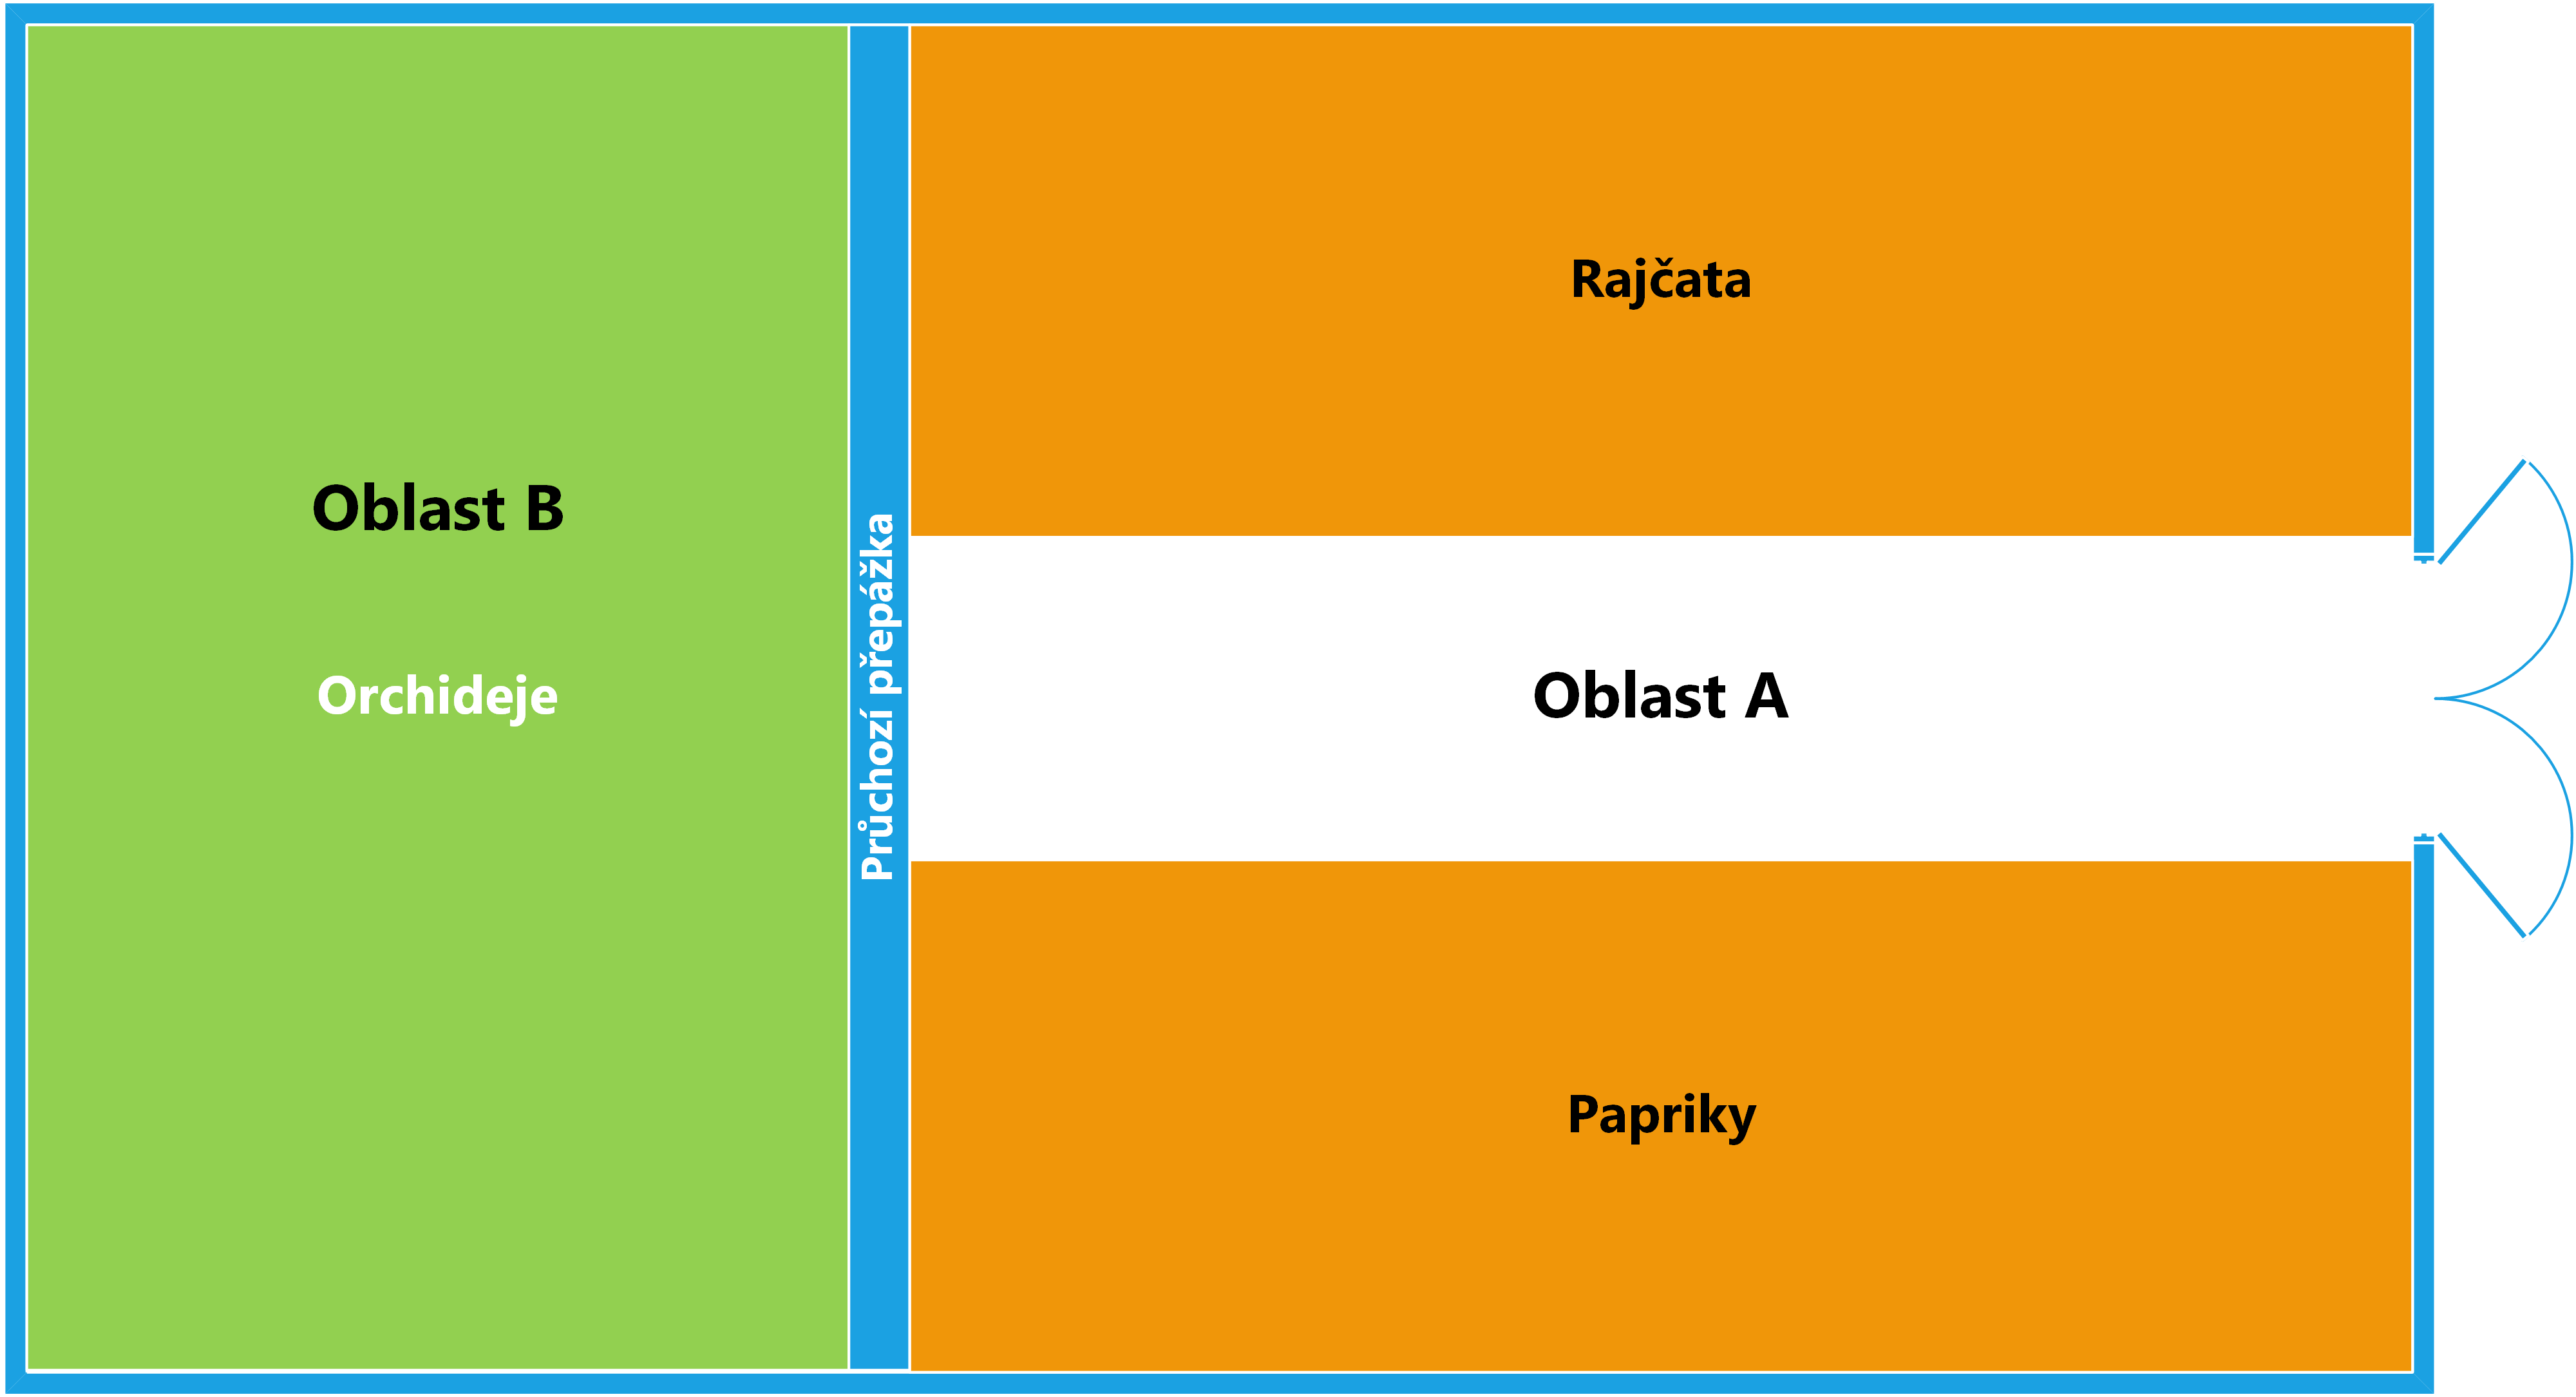
\includegraphics[width=0.85\textwidth]{img/Rozdeleni_Skleniku_A.png}
    \caption{Rozdělení skleníku na dvě oblasti.}
    \label{fig:separationA}
\end{figure}

\newpage